% ***************************************************************************************************
%
%	Szablon pracy magisterskiej dla Politechniki Wrocławskiej w wersji dwustronnej.
%	Autor:	Tomasz Strzałka
% Koretkta i dostosowanie do wymogów WIT 3.12.2021: dr inż. Anna Lauks-Dutka
%
% ***************************************************************************************************

% Styl dwustronny z domyślną wielkością czcionki 10pt oraz oddzieloną stroną tytułową (titlepage).
% Domyślnie rodziały rozpoczynają się na stronie prawej (openright).
\documentclass[10pt]{book}
\usepackage{times}


% ***************************************************************************************************
% Ustawienia języka
% ***************************************************************************************************

% Podstawowe ustawienia języka, według którego formatowany będzie dokument
\usepackage[polish]{babel}

% Pakiet babel dla polskiego języka powoduje konflikt z pakietem amssymb.
% Polecenie '\lll' definiują oba pakiety - porządana jest druga definicja.
\let\lll\undefined

% W przypadku wielojęzykowości ustawia główny język dokumentu
\selectlanguage{polish}

% Kodowanie dokumentu
\usepackage[utf8]{inputenc}

% Dowolny rozmiar czcionek, kodowanie znaków
\usepackage{lmodern}

% Polskie wcięcia akapitów
\usepackage{indentfirst}

% Polskie łamanie wyrazów
\usepackage[plmath]{polski}

% Przecinek w wyrażeniach matematycznych zamiast kropki
\usepackage{icomma}

% Polskie formatowanie typograficzne
\frenchspacing

% Zapewnia liczne usprawnienia wyświetlania i organizacji matematycznych formuł. 
\usepackage{amsmath}

% Wprowadza rozszerzony zestaw symboli m.in. \leadsto
\usepackage{amssymb}

% Dodatkowa, ,,kręcona'' czcionka matematyczna
\usepackage{mathrsfs}

% Dodatkowe wsparcie dla środowiska mathbb, które nie wspiera domyślnie cyfr (\mathbb{})
\usepackage{bbold}

% Fixes/improves amsmath
\usepackage{mathtools}


% ***************************************************************************************************
% Kolory  
% ***************************************************************************************************

% Umożliwia kolorowanie poszczególnych komórek tabeli
\usepackage[table]{xcolor}% http://ctan.org/pkg/

% Umożliwia łatwą zmianę koloru linii w tabeli
\usepackage{tabu}

% Umożliwia rozszerzoną kontrolę nad kolorami.
\usepackage{xcolor}

% Definicje kolorów
\definecolor{lgray}{HTML}{9F9F9F}
\definecolor{dgray}{HTML}{5F5F5F}
% lgray				-	nazwa nowo zdefiniowanego koloru
% HTML				-	model kolorów
% CCCCCC			-	wartość koloru zgodna z modelem

% ***************************************************************************************************
% Algorytmy 
% ***************************************************************************************************

% Udostępnia środowisko do konstruowania pseudokodów
\usepackage[ruled,vlined,linesnumbered,longend,algochapter]{algorithm2e}
% ruled	- poziome kreski na początku i końcu algorytmu, podpis na górze oddzielony również kreską poziomą
% vlined - pionowe kreski łączące początek polecenia z jego końcem
% linesnumbered	- numerowanie kolejnych wierszy algorytmu
% longend - długie końcówki np. ifend, forend itd.
% algochapter - numeracja z rozdziałami

% Zamiana nazwy środowiska z domyślnej "Algorithm X" na "Pseudokod X"
\newenvironment{pseudokod}[1][htb]{
	\renewcommand{\algorithmcfname}{Pseudokod}
	\begin{algorithm}[#1]%
	}{
\end{algorithm}
}

% Zmiana rozmiaru komentarzy
\newcommand\algcomment[1]{
	\footnotesize{#1}
}

% Ustawienie zadanego stylu dla komentarzy
\SetCommentSty{algcomment}

% Wyśrodkowana tylda
\usepackage{textcomp}%
\newcommand{\textapprox}{\raisebox{0.5ex}{\texttildelow}}

% Listowanie kodów źródłowych
\usepackage{listings} 
\renewcommand{\lstlistingname}{Kod źródłowy} % Polska nazwa listingu

% Definicje specjalnych znaków, które nie są obsługiwane w środowisku listing
\lstset{literate=
	{ż}{{\.{z}}}1	{ź}{{\'{z}}}1
	{ć}{{\'{c}}}1	{ń}{{\'{n}}}1
	{ą}{{\c a}}1	{ś}{{\'{s}}}1
	{ł}{{\l}}1		{ę}{{\c{e}}}1
	{ó}{{\'{o}}}1	{á}{{\'a}}1
	{é}{{\'e}}1		{í}{{\'i}}1
	{ó}{{\'o}}1		{ú}{{\'u}}1
	{ù}{{\`u}}1		{Á}{{\'A}}1
	{É}{{\'E}}1		{Í}{{\'I}}1
	{Ó}{{\'O}}1		{Ú}{{\'U}}1
	{à}{{\`a}}1		{è}{{\'e}}1
	{ì}{{\`i}}1		{ò}{{\`o}}1
	{ò}{{\`o}}1		{À}{{\`A}}1
	{È}{{\'E}}1		{Ì}{{\`I}}1
	{Ò}{{\`O}}1		{Ò}{{\`O}}1
	{ä}{{\"a}}1		{ë}{{\"e}}1
	{ï}{{\"i}}1		{ö}{{\"o}}1
	{ü}{{\"u}}1		{Ä}{{\"A}}1
	{Ë}{{\"E}}1		{Ï}{{\"I}}1
	{Ö}{{\"O}}1		{Ü}{{\"U}}1
	{â}{{\^a}}1		{ê}{{\^e}}1
	{î}{{\^i}}1		{ô}{{\^o}}1
	{û}{{\^u}}1		{Â}{{\^A}}1
	{Ê}{{\^E}}1		{Î}{{\^I}}1
	{Ô}{{\^O}}1		{Û}{{\^U}}1
	{œ}{{\oe}}1		{Œ}{{\OE}}1
	{æ}{{\ae}}1		{Æ}{{\AE}}1
	{ß}{{\ss}}1		{ç}{{\c c}}1
	{Ç}{{\c C}}1	{ø}{{\o}}1
	{å}{{\r a}}1	{Å}{{\r A}}1
	{€}{{\EUR}}1	{£}{{\pounds}}1
}

% ***************************************************************************************************
% Marginesy 
% ***************************************************************************************************

% Ustawienia rozmiarów stron i ich marginesów
%korekta ALD - dodatkowe 0.5cm na oprawę z lewej
%\usepackage[headheight=18pt, top=25mm, bottom=25mm, left=25mm, right=25mm]{geometry}
\usepackage[headheight=18pt, top=25mm, bottom=25mm, left=30mm, right=25mm]{geometry}
% headheight		-	wysokość tytułów
% top				-	margines górny
% bottom			-	margines dolny
% left				-	margines lewy
% right				-	margines prawy

% Usunięcie górnego marginesu dla środowisk
\makeatletter
\setlength\@fptop{0\p@}	
\makeatother

% ***************************************************************************************************
% Styl 
% ***************************************************************************************************

% Definiuje środowisko 'titlingpage', które zapewnia pełną kontrolę nad układem strony tytułowej.
\usepackage{titling}


% Umożliwia modyfikowanie stylu spisu treści
\usepackage{tocloft}	

\tocloftpagestyle{tableOfContentStyle}

% Definiowanie własnych stylów nagłówków i/lub stopek
\usepackage{fancyhdr}

% Domyślny styl dla pracy 
\fancypagestyle{custom}{
	\fancyhf{}									% wyczyść stopki i nagłówki
	\fancyhead[RO]{								% Prawy, nieparzysty nagłówek
%korekta ALD: 
%\hrulefill \hspace{16pt} \large Rozdział \thechapter
		\hrulefill \hspace{16pt} \large \ifnum \thechapter>0 {Rozdział \thechapter} \else{Wstęp}\fi
		\put(-472.1, 12.1){%
			\makebox(0,0)[l]{%
                
\includegraphics[width=0.05\textwidth]{pwr-logo}
			}
		}
		\put(-443,5.5){%
			\makebox(0,0)[l]{%
				\small Politechnika Wrocławska
			}
		}
	}
	\fancyhead[LE]{								% Lewy, parzysty nagłówek
%korekta ALD: 
%\large Rozdział \thechapter \hspace{16pt} \hrulefill 
        \large \ifnum \thechapter>0 {Rozdział \thechapter} \else{Wstęp}\fi \hspace{16pt} \hrulefill 
		\put(-22, 12.1){%
			\makebox(0,0)[l]{%
                %korekta ALD
				%
\includegraphics[width=0.05\textwidth]{pwr-logo}
                
\includegraphics[width=0.05\textwidth]{wit-logo}			}
		}
		\put(-210,5.5){%
			\makebox(0,0)[l]{%
%				\small Wydział Podstawowych Problemów Techniki
%Korekta ALD
\small Wydział Informatyki i Telekomunikacji
			}
		}
	}
	\fancyfoot[LE,RO]{							% Stopki
		\thepage
	}
	\renewcommand{\headrulewidth}{0pt}			% Grubość linii w nagłówku
	\renewcommand{\footrulewidth}{0.2pt}		% Grubość linii w stopce
}


% Domyślny styl dla bibliografii
\fancypagestyle{bibliographyStyle}{
	\fancyhf{}									% wyczyść stopki i nagłówki
	\fancyhead[RO]{								% Prawy, nieparzysty nagłówek
		\hrulefill \hspace{16pt} \large Dodatek \thechapter
		\put(-472.1, 12.1){%
			\makebox(0,0)[l]{%
	
\includegraphics[width=0.05\textwidth]{pwr-logo}
			}
		}
		\put(-443,5.5){%
			\makebox(0,0)[l]{%
				\small Politechnika Wrocławska
			}
		}
	}
	\fancyhead[LE]{								% Lewy, parzysty nagłówek
		\large Bibliografia \hspace{16pt} \hrulefill 
		\put(-22, 12.1){%
			\makebox(0,0)[l]{%
			%korekta ALD	\includegraphics[width=0.05\textwidth]{wppt-logo}
			
\includegraphics[width=0.05\textwidth]{wit-logo}
			}
		}
		\put(-210,5.5){%
			\makebox(0,0)[l]{%
			%korekta ALD
				%\small Wydział Podstawowych Problemów Techniki
				\small Wydział Informatyki i Telekomunikacji
			}
		}
	}
	\fancyfoot[LE,RO]{							% Stopki
		\thepage
	}
	\renewcommand{\headrulewidth}{0pt}			% Grubość linii w nagłówku
	\renewcommand{\footrulewidth}{0.2pt}		% Grubość linii w stopce
}

% Domyślny styl dla spisu tabel i rysunków
\fancypagestyle{listOfTablesStyle}{
	\fancyhf{}									% wyczyść stopki i nagłówki
	\fancyhead[RO]{								% Prawy, nieparzysty nagłówek
		\hrulefill \hspace{16pt} \large Spis tabel
		\put(-472.1, 12.1){%
			\makebox(0,0)[l]{%
			
\includegraphics[width=0.05\textwidth]{pwr-logo}
			}
		}
		\put(-443,5.5){%
			\makebox(0,0)[l]{%
				\small Politechnika Wrocławska
			}
		}
	}
	\fancyhead[LE]{								% Lewy, parzysty nagłówek
		\large Spis tabel \hspace{16pt} \hrulefill 
		\put(-22, 12.1){%
			\makebox(0,0)[l]{%

\includegraphics[width=0.05\textwidth]{wit-logo}
			}
		}
		\put(-210,5.5){%
			\makebox(0,0)[l]{%
				\small Wydział Informatyki i Telekomunikacji
			}
		}
	}
	\fancyfoot[LE,RO]{							% Stopki
		\thepage
	}
	\renewcommand{\headrulewidth}{0pt}			% Grubość linii w nagłówku
	\renewcommand{\footrulewidth}{0.2pt}		% Grubość linii w stopce
}

\fancypagestyle{listOfPlotsStyle}{
	\fancyhf{}									% wyczyść stopki i nagłówki
	\fancyhead[RO]{								% Prawy, nieparzysty nagłówek
		\hrulefill \hspace{16pt} \large Spis rysunków
		\put(-472.1, 12.1){%
			\makebox(0,0)[l]{%
			
\includegraphics[width=0.05\textwidth]{pwr-logo}
			}
		}
		\put(-443,5.5){%
			\makebox(0,0)[l]{%
				\small Politechnika Wrocławska
			}
		}
	}
	\fancyhead[LE]{								% Lewy, parzysty nagłówek
		\large Spis rysunków \hspace{16pt} \hrulefill 
		\put(-22, 12.1){%
			\makebox(0,0)[l]{%

\includegraphics[width=0.05\textwidth]{wit-logo}
			}
		}
		\put(-210,5.5){%
			\makebox(0,0)[l]{%
				\small Wydział Informatyki i Telekomunikacji
			}
		}
	}
	\fancyfoot[LE,RO]{							% Stopki
		\thepage
	}
	\renewcommand{\headrulewidth}{0pt}			% Grubość linii w nagłówku
	\renewcommand{\footrulewidth}{0.2pt}		% Grubość linii w stopce
}

% Domyślny styl dla dodatków
\fancypagestyle{appendixStyle}{
	\fancyhf{}									% wyczyść stopki i nagłówki
	\fancyhead[RO]{								% Prawy, nieparzysty nagłówek
		\hrulefill \hspace{16pt} \large Załącznik \thechapter
		\put(-472.1, 12.1){%
			\makebox(0,0)[l]{%

\includegraphics[width=0.05\textwidth]{pwr-logo}
			}
		}
		\put(-443,5.5){%
			\makebox(0,0)[l]{%
				\small Politechnika Wrocławska
			}
		}
	}
	\fancyhead[LE]{								% Lewy, parzysty nagłówek
		\large Załącznik \thechapter \hspace{16pt} \hrulefill 
		\put(-22, 12.1){%
			\makebox(0,0)[l]{%
%korekta ALD:				\includegraphics[width=0.05\textwidth]{wppt-logo}

\includegraphics[width=0.05\textwidth]{wit-logo}
			}
		}
		\put(-210,5.5){%
			\makebox(0,0)[l]{%
			%korekta ALD
				%\small Wydział Podstawowych Problemów Techniki
				\small Wydział Informatyki i Telekomunikacji
			}
		}
	}
	\fancyfoot[LE,RO]{							% Stopki
		\thepage
	}
	\renewcommand{\headrulewidth}{0pt}			% Grubość linii w nagłówku
	\renewcommand{\footrulewidth}{0.2pt}		% Grubość linii w stopce
}

% Osobny styl dla stron zaczynających rozdział/spis treści itd. (domyślnie formatowane jako "plain")
\fancypagestyle{chapterBeginStyle}{
	\fancyhf{}%
	\fancyfoot[LE,RO]{
		\thepage
	}
	\renewcommand{\headrulewidth}{0pt}
	\renewcommand{\footrulewidth}{0.2pt}
}

% Styl dla pozostałych stron spisu treści
\fancypagestyle{tableOfContentStyle}{
	\fancyhf{}%
	\fancyfoot[LE,RO]{
		\thepage
	}
	\renewcommand{\headrulewidth}{0pt}
	\renewcommand{\footrulewidth}{0.2pt}
}
% Formatowanie tytułów rozdziałów i/lub sekcji
\usepackage{titlesec}

% Formatowanie tytułów rozdziałów
\titleformat{\chapter}[hang]					% kształt
{
	\vspace{-10ex}
	%\Huge
	\large
	\bfseries
}												% formatowanie tekstu modyfikowanego elementu
{}												% etykieta występująca przed tekstem modyfikowanego elementu, niewidoczna w spisie treści
{
	10pt
}												% odstęp formatowanego tytułu od lewego marginesu/etykiety
{
    \large
	\bfseries
}												% formatowanie elementów przed modyfikowanym tytułem
[
\vspace{2ex}
%\rule{\textwidth}{0.4pt}
%\vspace{-4ex}
]												% dodatkowe formatowanie stosowane poniżej modyfikowanego tytułu


% Formatowanie tytułów sekcji
\titleformat{\section}[hang]					% kształt
{
	\vspace{2ex}
%	\titlerule\vspace{1ex}
	\large\bfseries
}												% formatowanie tekstu modyfikowanego elementu
{
	\thesection									% etykieta występująca przed tekstem modyfikowanego elementu, niewidoczna w spisie treści
}
{
	0pt
}												% odstęp formatowanego tytułu od lewego marginesu/etykiety
{
	\large
	\bfseries
}												% formatowanie elementów przed modyfikowanym tytułem


%ALD- ustawienia wielkości fontów dla rozdziałów i sekcji
\usepackage{sectsty}
%\chapterfont{\fontsize{14}{17.6}\selectfont}
\sectionfont{\fontsize{13}{16.8}\selectfont}
\subsectionfont{\fontsize{12}{15.6}\selectfont}

% ***************************************************************************************************
% Linki
% ***************************************************************************************************

% Umożliwia wstawianie hiperłączy do dokumentu
\usepackage{hyperref}							% Aktywuje linki

\hypersetup{
	colorlinks	=	true,					% Koloruje tekst zamiast tworzyć ramki.
	linkcolor		=	blue,					% Kolory: referencji,
        citecolor		=	blue,					% cytowań,
	urlcolor		=	blue					% hiperlinków.
}

% Do stworzenia hiperłączy zostanie użyta ta sama (same) czcionka co dla reszty dokumentu
\urlstyle{same}




% ***************************************************************************************************
% Linki
% ***************************************************************************************************

% Umożliwia zdefiniowanie własnego stylu wyliczeniowego
\usepackage{enumitem}

% Nowa lista numerowana z trzema poziomami
\newlist{myitemize}{itemize}{3}

% Definicja wyglądu znacznika pierwszego poziomu
\setlist[myitemize,1]{
	label		=	\textbullet,
	leftmargin	=	4mm}

% Definicja wyglądu znacznika drugiego poziomu
\setlist[myitemize,2]{
	label		=	$\diamond$,
	leftmargin	=	8mm}

% Definicja wyglądu znacznika trzeciego poziomu
\setlist[myitemize,3]{
	label		=	$\diamond$,
	leftmargin	=	12mm
}

% ***************************************************************************************************
% Inne pakiety
% ***************************************************************************************************

% Dołączanie rysunków
\usepackage{graphicx}

% Figury i przypisy
\usepackage{caption}
\usepackage{subcaption}

% Umożliwia tworzenie przypisów wewnątrz środowisk
\usepackage{footnote}

% Umożliwia tworzenie struktur katalogów
\usepackage{dirtree}

% Rozciąganie komórek tabeli na wiele wierszy
\usepackage{multirow}

% Precyzyjne obliczenia szerokości/wysokości dowolnego fragmentu wygenerowanego przez LaTeX
\usepackage{calc}

% ***************************************************************************************************
% Matematyczne skróty
% ***************************************************************************************************

% Skrócony symbol liczb rzeczywistych
\newcommand{\RR}{\mathbb{R}}

% Skrócony symbol liczb naturalnych
\newcommand{\NN}{\mathbb{N}}

% Skrócony symbol liczb wymiernych
\newcommand{\QQ}{\mathbb{Q}}

% Skrócony symbol liczb całkowitych
\newcommand{\ZZ}{\mathbb{Z}}

% Skrócony symbol logicznej implikacji
\newcommand{\IMP}{\rightarrow}

% Skrócony symbol  logicznej równoważności
\newcommand{\IFF}{\leftrightarrow}

% ***************************************************************************************************
% Środowiska
% ***************************************************************************************************

% Środowisko do twierdzeń
\newtheorem{theorem}{Twierdzenie}[chapter]

% Środowisko do lematów
\newtheorem{lemma}{Lemat}[chapter]

% Środowisko do przykładów
\newtheorem{example}{Przykład}[chapter]

% Środowisko do wniosków
\newtheorem{corollary}{Wniosek}[chapter]

% Środowisko do definicji
\newtheorem{definition}{Definicja}[chapter]

% Środowisko do dowodów
\newenvironment{proof}{
	\par\noindent \textbf{Dowód.}
}{
\begin{flushright}
	\vspace*{-6mm}\mbox{$\blacklozenge$}
\end{flushright}
}

%ALD - nowe środowisko do streszczenia i abstractu
\newenvironment{streszczenie}{
	\par\noindent {\large \textbf{Streszczenie}\\[14pt]\indent}
}{}
\newenvironment{abstract}{
	\par\noindent {\large \textbf{Abstract}\\[14pt]\indent}
}{}

% Środowisko do uwag
\newenvironment{remark}{
	\bigskip \par\noindent \small \textbf{Uwaga.}
}{
\begin{small}
	\vspace*{4mm}
\end{small}
}

% ***************************************************************************************************
% Słownik
% ***************************************************************************************************

% Prawidłowe dzielenie wyrazów
\hyphenation{wszy-stkich ko-lu-mnę każ-da od-leg-łość
	dzie-dzi-ny dzie-dzi-na rów-nych rów-ny
	pole-ga zmie-nna pa-ra-met-rów wzo-rem po-cho-dzi
	o-trzy-ma wte-dy wa-run-ko-wych lo-gicz-nie
	skreś-la-na skreś-la-ną cał-ko-wi-tych wzo-rów po-rzą-dek po-rząd-kiem
	przy-kład pod-zbio-rów po-mię-dzy re-pre-zen-to-wa-ne
	rów-no-waż-ne bi-blio-te-kach wy-pro-wa-dza ma-te-ria-łów
	prze-ka-za-nym skoń-czo-nym moż-esz na-tu-ral-na cią-gu tab-li-cy
	prze-ka-za-nej od-po-wied-nio}

% ***************************************************************************************************
% Dokument
% ***************************************************************************************************

\frontmatter

\begin{document}

    \pagestyle{empty}
	\begin{titlingpage}
		\vspace*{\fill}
		\begin{center}
			\begin{picture}(430,500)
				\put(60,590){\makebox(0,0)[l]{\huge \textbf{Politechnika Wrocławska}}}
				\put(40,565){\makebox(0,0)[l]{\Large \textbf{Wydział Informatyki i Telekomunikacji}}}
                \put(0,550){\line(1,0){430}}
                \put(0,510){\makebox(0,0)[l]{\large Kierunek: \textbf{INA}}}
                %\textbf{3 literowy kod kierunku}}}
                \put(0,490){\makebox(0,0)[l]{\large Specjalność: \textbf{-}}}                
                %\textbf{3 literowy kod specjalności}}}                
				\put(0,370){\begin{minipage}{0.9\textwidth}
				\centering
				\Huge \textsc{Praca Dyplomowa\\ Inżynierska}
                \end{minipage}
				}
% Tytuł pracy
				\put(0,230){\begin{minipage}{0.9\textwidth}
				\centering
				\LARGE \textbf{Algorytm Minimax do gry w Warcaby}
                \end{minipage}
				}
% Autor pracy
				\put(0,170){\begin{minipage}{0.9\textwidth}
				\centering
				\Large {
				Janusz Witkowski
				}
				\end{minipage}
				}
% dane promotora
				\put(0,90){\begin{minipage}{0.9\textwidth}
				\centering
				\large{
				Opiekun pracy\\
				\textbf{dr Maciej Gębala}
				}
				\end{minipage}
				}
				\put(0,-30){
				\begin{minipage}{0.9\textwidth}
				\normalsize{
				Sztuczna inteligencja, Algorytmika, Algorytmy metaheurystyczne, Teoria gier 
				}
				\end{minipage}
				}
                \put(0,-80){\line(1,0){430}}
				\put(155,-100){\makebox(0,0)[bl]{\large \textsc{Wrocław 2022}}}
			\end{picture}
		\end{center}	
		\vspace*{\fill}
	\end{titlingpage}
	
    \cleardoublepage
	\begin{streszczenie}
W pracy zaimplementowano algorytm Minimax z cięciami alfa-beta do gry w~warcaby w~wariancie angielskim. Algorytm używa funkcji oceny heurystycznej rozpatrującej parametry danego stanu rozgrywki. Do wyznaczenia odpowiednich priorytetów parametrów wykorzystano algorytm genetyczny. 
\end{streszczenie}

	\vspace*{1cm}	
    \begin{abstract}
The thesis is concentrated on implementing Minimax algorithm with alpha-beta-pruning for the game of English draughts (American Checkers). It involves a heuristic function which considers some number of parameters of given game state. To find suitable priorities for these parameters, a genetic algorithm was used.
\end{abstract}

% W pracy zaimplementowano algorytm Minimax z cięciami alfa-beta do gry w warcaby w wariancie angielskim. Algorytm używa funkcji oceny heurystycznej rozpatrującej parametry danego stanu rozgrywki. Do wyznaczenia odpowiednich priorytetów parametrów wykorzystano algorytm genetyczny. 

    \cleardoublepage
	\pagenumbering{Roman}
	\pagestyle{tableOfContentStyle}
	\tableofcontents

	% spis rysunków (opcjonalnie)    
	\clearpage
	\pagestyle{listOfPlotsStyle}
        \listoffigures
        \addcontentsline{toc}{chapter}{Spis rysunków}
        
        % spis tabel (opcjonalnie)
        \clearpage
        \renewcommand{\listtablename}{Spis tabel}    
        \pagestyle{listOfTablesStyle}
	\listoftables
	\addcontentsline{toc}{chapter}{Spis tabel}




    \cleardoublepage
    
		
	% ***************************************************************************************************
	% Wstęp
	% ***************************************************************************************************
	
	\pagestyle{custom}
	\mainmatter
	
	% ***************************************************************************************************
	% Rodziały
	% ***************************************************************************************************

	%Korekta ALD - nienumerowany wstęp
%\chapter{Wstęp}
\addcontentsline{toc}{chapter}{Wstęp}
\chapter*{Wstęp}

\thispagestyle{chapterBeginStyle}

{\color{dgray}
We wstępie zostanie zawarte tak zwane ``lanie wody". Najprawdopodobniej będzie to część dokumentu która swój ostateczny obraz obierze pod sam koniec pisania. Aby dobrze wprowadzić Czytelników w temat pracy, autor musi mieć przed oczyma całość swojego dzieła.

Pierwsza wersja tejże pisemnej pracy dyplomowej posiada wyszczególnione rozdziały i podrozdziały, wraz ze szczątkowym opisem ich przyszłej zawartości. 

% Reszta rozdziału ``Wstęp" pozostanie na moment w tym samym stanie jak w szablonie pracy WIT.

% Wstęp pracy (nie numerowany) powinien składać się z czterech części (które nie są wydzielane jako osobne podrozdziały): zakresu pracy, celu, analizy i porównania istniejących rozwiązań oraz przeglądu literatury, oraz opisu zawartości pracy.

% Każdy rozdział powinien rozpoczynać się od akapitu wprowadzającego, w którym zostaje w skrócie omówiona zawartość tego rozdziału.
}



% {\color{dgray}
% Praca swoim zakresem obejmuje wielowarstwowe rozproszone systemy informatyczne typu ,,B2B'' wspierające wymianę danych pomiędzy przedsiębiorstwami. Systemy tego typu, konstruowane dla dużych korporacji, charakteryzują się złożoną strukturą poziomą i pionową, w której dokumenty \ldots

% Celem pracy jest zaprojektowanie i oprogramowanie aplikacji o następujących założeniach funkcjonalnych:
% \begin{itemize}
%     \item wspieranie zarządzania obiegiem dokumentów wewnątrz korporacji z uwzględnieniem \ldots,
% 	\item wspieranie zarządzania zasobami ludzkimi z uwzględnieniem modułów kadrowych oraz \ldots,
% 	\item gotowość do uzyskania certyfikatu ISO \ldots,
% 	\item \ldots.
% \end{itemize}

% Istnieje szereg aplikacji o zbliżonej funkcjonalności: \ldots, przy czym \ldots.

% Praca składa się z czterech rozdziałów.
% W rozdziale pierwszym omówiono strukturę przedsiębiorstwa \ldots, scharakteryzowano grupy użytkowników oraz przedstawiono procedury związane z obiegiem dokumentów. Szczegółowo opisano mechanizmy \ldots. Przedstawiono uwarunkowania prawne udostępniania informacji \ldots, w ramach \ldots.

% W rozdziale drugim przedstawiono szczegółowy projekt systemy w notacji UML. Wykorzystano diagramy \ldots.
% Opisano w pseudokodzie i omówiono algorytmy generowania \ldots.

% W rozdziale trzecim opisano technologie implementacji projektu: wybrany język programowania, biblioteki, system zarządzania bazą danych, itp.  Przedstawiono dokumentację techniczną kodów źródłowych interfejsów poszczególnych modułów systemu. Przedstawiono sygnatury metod publicznych oraz \ldots.

% W rozdziale czwartym przedstawiono sposób instalacji i wdrożenia systemu w środowisku docelowym.

% Końcowy rozdział stanowi podsumowanie uzyskanych wyników.
% }


	\cleardoublepage

	\chapter{Warcaby}
\thispagestyle{chapterBeginStyle}
\label{rozdzial1}

% {\color{dgray}
% Niniejszy rozdział poświęcony będzie zaznajomieniu Czytelnika z grą w Warcaby oraz szczególną wersją tej gry. Omówione również zostaną powody skupienia się nad tym wariantem, jak i inne badania przeprowadzone w przeszłości przez naukowców.
% }

% Warcaby są jedną z najpopularniejszych klasycznych gier dwuosobowych. Jest to przedstawiciel gier o doskonałej informacji, tj. gracze na każdym stadium gry posiadają pełną wiedzę na temat sytuacji na planszy oraz historii ruchów. Zaliczają się też do gier o sumie zerowej, czyli takich w których zysk jednego gracza przekłada się bezpośrednio na stratę drugiego, a zwycięzca może być tylko jeden. \ldots

Warcaby to jedna z najpopularniejszych klasycznych gier dwuosobowych, zaliczanych do gier z doskonałą informacją i gier o sumie zerowej. Przyjmuje się, że gra ta zrodziła się w XII wieku, najprawdopodobniej na południu Francji lub w Hiszpanii, oraz że wywodzi się ona z dawnej arabskiej gry Alquerque~\cite{Gry}. Istnieją coroczne turnieje i mistrzostwa światowe w różnych odmianach Warcabów, choć dzięki nieskomplikowanym zasadom są one popularne również w mniejszych kręgach.

\section{Reguły warcabów standardowych}

Pojedynczą partię Warcabów rozgrywa się na szachownicy 8x8 o polach na zmianę pomalowanych na jasno lub ciemno. W grze wykorzystywane są dwa rodzaje figur - piony i damki. Obydwaj gracze rozstawiają po 12 pionów na ciemnych polach w swoich pierwszych trzech rzędach. Dla rozróżnienia, piony pierwszego gracza są koloru białego, natomiast piony drugiego gracza - czarnego. Celem gry jest wyeliminowanie wszystkich figur przeciwnika lub zablokowanie go, poprzez serię naprzemiennych ruchów swoimi figurami. (Zablokowanie gracza oznacza doprowadzenie do takiej sytuacji, w której gracz ten nie jest w stanie wykonać żadnego legalnego ruchu w momencie gdy następuje jego kolej.)

\FloatBarrier

% \hspace{5cm}

\begin{figure}[h!]
\centering
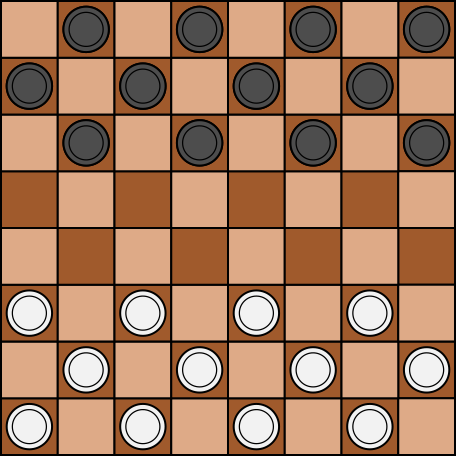
\includegraphics[scale=.6]{graphics/warcaby_planszaStartowa.png}
\caption{Stan początkowy planszy w Warcabach.}
\label{fig:plansza}
\end{figure}

\FloatBarrier

Wszystkie figury w grze mogą poruszać się tylko i wyłącznie na ukos (przez co żadne jasne pole na planszy nie zostanie zajęte przez żadną figurę w trakcie rozgrywki). Piony z którymi zaczynają gracze poruszają się tylko o jedno pole w przód względem ich właściciela. Tzn. pion może skoczyć na pole ukośnie sąsiadujące w kierunku oponenta, o ile pole to nie jest zajęte przez inną figurę. W grze istnieje również druga figura - jeżeli pion gracza dojdzie do końca planszy znajdującego się po stronie jego oponenta (do tzw. rzędu awansu), pion zamieniany jest na damkę. Damka jest najpotężniejszą figurą w grze, jako że potrafi poruszyć się we wszystkich czterech kierunkach na ukos, a na dodatek przebyć dowolną liczbę pól w linii w jednym ruchu. Pod tym względem damkę najłatwiej porównać z figurą gońca w szachach.

Każdą figurę w Warcabach można zbijać, tj. usuwać z obecnej rozgrywki. Piony mogą zbijać sąsiednie figury przeciwnika, wykonując skok nad tą figurą na następne pole w linii prostej, o ile takie pole jest wolne. Piony mogą bić zarówno do przodu, jak i do tyłu. Damki w standardowych Warcabach zbijają ze znacznie większego dystansu (można powiedzieć, że w momencie zbijania ich "sąsiadowanie" z przeciwnymi figurami nie jest ograniczone do jednego pola różnicy). Zbita figura zostaje zdjęta z planszy i nie bierze udziału w rozgrywce do momentu jej zakończenia. Nie można bić swoich figur.

Bicia w Warcabach mają specjalne reguły wyróżniające je spośród innych gier planszowych. Po pierwsze, w jednym ruchu jedna figura może wykonać wiele bić. Jeśli po jednym biciu figura wskoczyła w miejsce z którego jest w stanie przeprowadzić kolejne bicie, można takie bicie wykonać w tej samej turze. W jednym ruchu nie można dwa razy zbić tej samej figury. Po drugie, bicia są obowiązkowe. Jeżeli gracz w swojej turze jest postawiony w sytuacji w której co najmniej jedna z jego figur ma możliwość bicia, gracz ten musi wykonać taki ruch. Dodatkowo, o ile ruch bicia pionem można wybrać w przypadku większej liczby możliwych bić, damki mają obowiązek maksymalnego bicia, tj. należy przeprowadzić bicie o największej możliwej liczbie zbijanych figur w jednym ruchu.

\section{Wariant angielski}

\FloatBarrier

Praca skupiona jest na szczególnej wersji gry w Warcaby, nazywanej na ogół wariantem angielskim, lub w niektórych kręgach wariantem amerykańskim. Został on wybrany głównie ze względu na ograniczenie przestrzeni stanów w jakich może znaleźć się rozgrywka - reguły gry dostosowane do tego wariantu znacznie zmniejszają liczbę możliwości które rozgrywający algorytm musi rozpatrzeć.

% \subsection{Zmiany w zasadach}

Wariant ten wprowadza dwie zmiany do zasad gry względem wariantu standardowego (opierając się o~\cite{Gry}). Po pierwsze, zwykłe piony nie mogą bić do tyłu. Po drugie, damkom ogranicza się możliwość ruchu o dowolną liczbę pól do jednego sąsiedniego pola oraz do bicia wyłącznie sąsiadujących przeciwnych figur, lecz wciąż mogą poruszać się we wszystkich kierunkach na ukos. Jedyną przewagą damek nad pionkami w tym wariancie jest możliwość ruchu i bicia do tyłu.

% \begin{figure}
% \centering
% \begin{minipage}{.5\textwidth}
%     \centering
%     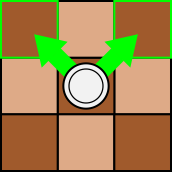
\includegraphics[scale=.6]{graphics/warcaby_ruchyPionZwykle.png}
%     \captionof{figure}{Ruchy piona w wariancie angielskim}
%     \label{fig:sub1}
% \end{minipage}%
% \begin{minipage}{.5\textwidth}
%     \centering
%     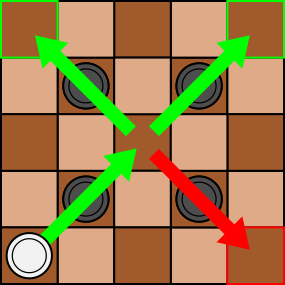
\includegraphics[scale=.6]{graphics/warcaby_ruchyPionBicia.png}
%     \captionof{figure}{Bicia piona w wariancie angielskim}
%     \label{fig:sub2}
% \end{minipage}
% \end{figure}

% \begin{figure}
% \centering
% \begin{minipage}{.5\textwidth}
%     \centering
%     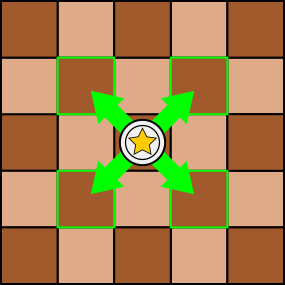
\includegraphics[scale=.6]{graphics/warcaby_ruchyDamkaZwykle.png}
%     \captionof{figure}{Ruchy damki w wariancie angielskim}
%     \label{fig:sub1}
% \end{minipage}%
% \begin{minipage}{.5\textwidth}
%     \centering
%     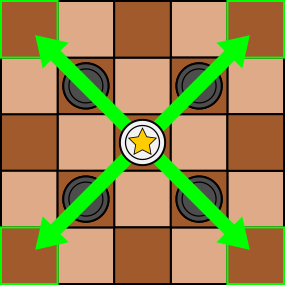
\includegraphics[scale=.6]{graphics/warcaby_ruchyDamkaBicia.png}
%     \captionof{figure}{Bicia damki w wariancie angielskim}
%     \label{fig:sub2}
% \end{minipage}
% \end{figure}

\begin{figure}
\centering
\begin{subfigure}{.5\textwidth}
  \centering
  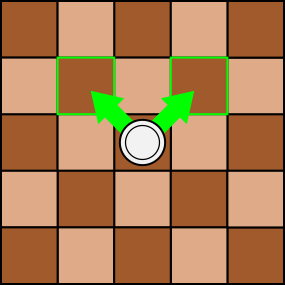
\includegraphics[scale=.6]{graphics/warcaby_ruchyPionZwykle3.png}
  \caption{Legalne ruchy}
  \label{fig:sub1}
\end{subfigure}%
\begin{subfigure}{.5\textwidth}
  \centering
  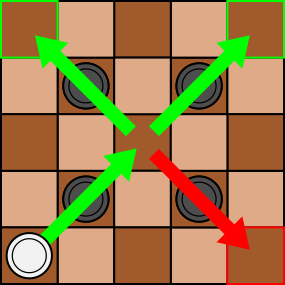
\includegraphics[scale=.6]{graphics/warcaby_ruchyPionBicia.png}
  \caption{Legalne bicia}
  \label{fig:sub2}
\end{subfigure}
\caption{Zestaw możliwych ruchów dla piona w wariancie angielskim}
\label{fig:test}
\end{figure}

\begin{figure}
\centering
\begin{subfigure}{.5\textwidth}
  \centering
  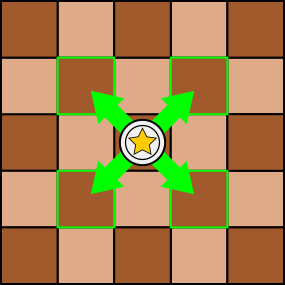
\includegraphics[scale=.6]{graphics/warcaby_ruchyDamkaZwykle.png}
  \caption{Legalne ruchy}
  \label{fig:sub11}
\end{subfigure}%
\begin{subfigure}{.5\textwidth}
  \centering
  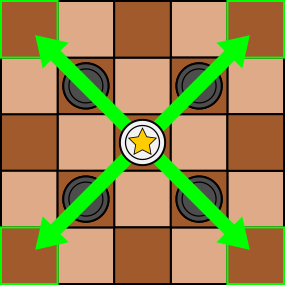
\includegraphics[scale=.6]{graphics/warcaby_ruchyDamkaBicia.png}
  \caption{Legalne bicia}
  \label{fig:sub22}
\end{subfigure}
\caption{Zestaw możliwych ruchów dla damki w wariancie angielskim}
\label{fig:test}
\end{figure}

\FloatBarrier

Przydatna w implementacji rzecz o której warto wspomnieć jest rozpatrywanie remisów. W grach towarzyskich remis zazwyczaj następuje za obopólną zgodą graczy. Na arenie turniejowej istnieje parę kryteriów determinujących remis. W rozpatrywanej wersji wariantu angielskiego wykorzystywana będzie zasada 40 ruchów, która mówi że rozgrywka kończy się remisem w momencie gdy w 40 naprzemiennych ruchach obu graczy nie została zbita ani jedna figura.

\FloatBarrier

\subsection{Badania wariantu}

Do rozwoju badań nad Warcabami w wariancie angielskim najmocniej przyczynił się Jonathan Schaeffer, profesor Uniwersytetu Alberty w Kanadzie. Jego zespół opracował Chinook'a, przeszukujący w głąb program do grania w Warcaby angielskie, który w roku 1992 oraz 1994 stanął naprzeciw ówczesnego mistrza świata Marion'a Tinsley'a i ogłoszony został pierwszym komputerowym zwycięzcą mistrzostw~\cite{Chinook}. Następnie, z pomocą programu, udowodnili poprzez słabe rozwiązanie (\textit{weakly solved}, pojęcie omówione w~\cite{Solving}) że każda gra w Warcabach angielskich kończy się remisem, pod warunkiem że gracze wykonują ruchy doskonale~\cite{Solved}. Pomimo uproszczonych zasad względem klasycznej wersji, wariant angielski posiada przestrzeń stanów wielkości rzędu $10^{20}$, dlatego też rozwiązanie zajęło zespołowi Schaeffer'a około 18 lat i 200 równolegle liczących maszyn.




	\cleardoublepage

	\chapter{Idea rozwiązania i algorytmy}
\thispagestyle{chapterBeginStyle}
\label{rozdzial2}

% {\color{dgray}
% W tym rozdziale przedstawione zostanie podejście autora do problemu opisanego w rozdziale~\ref{rozdzial1}. Każdy omawiany aspekt podejścia i każda idea wykorzystywanych algorytmów podparta zostanie pseudokodem bądź ilustracją, jeżeli zajdzie taka potrzeba.
% }

Głównym celem pracy jest stworzenie prostego modelu sztucznej inteligencji do grania w Warcaby w wariancie angielskim z pewną strategią. Istnieją różne podejścia do tego zagadnienia, spośród których najpopularniejszymi są te stosujące sieci neuronowe (zestawem danych byłaby np. baza meczów rozegranych na mistrzostwach na przestrzeni kilkunastu lat). Praca skupia się na bardziej nadzorowanej metodzie. Zastosowana została taktyka algorytmu Minimax połączonego z funkcją oceny heurystycznej. Do częściowego wyznaczenia funkcji oceny wykorzystano metodę algorytmu genetycznego.

\section{Minimax}

Minimax jest szczególną wersją algorytmu przeszukującego w grafie. Jego idea jest bardzo prosta i zbliżona do ludzkiego rozumowania. Mając dany stan planszy oraz głębokość przeszukiwania, algorytm rekurencyjnie rozpatruje kolejne stany planszy symulując wykonanie jednego możliwego ruchu. Kiedy już osiągnie maksymalną głębokość przeszukiwań, funkcją oceny heurystycznej przypisuje wartości stanom, po czym zwraca tę wartość do swojego stanu-rodzica. Mając wartości oceny od każdego swojego dziecka, stan wybiera jedną z nich i przekazuje ją do swojego rodzica. Gdy wybór dojdzie do stanu będącego korzeniem drzewa przeszukiwań, algorytm wybierze jedną z dostępnych mu ocen i zwróci ruch do stanu któremu ta ocena odpowiada.

{\small
\begin{pseudokod}[H]
%\SetAlTitleFnt{small}
\SetArgSty{normalfont}
\SetKwFunction{Evaluate}{evaluateState}
\SetKwFunction{Children}{getChildren}
\SetKwFunction{Minimax}{minimax}
\KwIn{Stan gry $state$, flaga gracza $maximizing$, głębokość przeszukiwań $h$, rozpatrujący gracz $player$}
\KwOut{Wartość funkcji oceny $eval$}
\eIf{$h = 0$}{
$eval \leftarrow \Evaluate{state, player}$\;
}{
\eIf{$maximizing = True$}{
$maxEval \leftarrow -\infty$\;
\ForEach{$child \in \Children{state}$}{
$childEval \leftarrow \Minimax{child, False, h - 1, player}$\;
\If{$childEval \ge maxEval$}{
$maxEval \leftarrow childEval$
% $bestState \leftarrow child$
}
}
% $state \leftarrow bestState$
$eval \leftarrow maxEval$
}{
$minEval \leftarrow +\infty$\;
\ForEach{$child \in \Children{state}$}{
$childEval \leftarrow \Minimax{child, True, h - 1, player}$\;
\If{$childEval \le minEval$}{
$minEval \leftarrow childEval$
% $bestState \leftarrow child$
}
}
% $state \leftarrow bestState$
$eval \leftarrow minEval$
}
}
% \ForEach{$b \in B$}{
% \Process{$b$}\;
% \For{$i \leftarrow 1$ \KwTo $|B|$}{
% \If{\Calculate{EW($i$,$b$)} $\le$ 0}{
% $b \leftarrow 2*b$\;
% }
% }
% }
% \While{$B \neq \emptyset$}{
% \For{$j \leftarrow 1$ \KwTo $|B|$}{
% \If{\Calculate{FT($j$,$\hat{b}$)} $\le 0$}{
% $w \leftarrow 2*\hat{b}$\;
% $W \leftarrow W \cup \{w\}$\;
% $B \leftarrow B \setminus \{b\}$\;
% }
% }
% }
\caption{Prosty algorytm Minimax}\label{alg:mine}
\end{pseudokod}
}

Swoją nazwę algorytm zawdzięcza naprzemiennemu rozpatrywaniu ocen heurystycznych w drzewie przeszukiwań. W momencie gdy dany gracz wywołuje procedurę Minimaxa rozpatrując możliwe do wykonania przez niego ruchy, oznaczany jest jako gracz MAX. W powstałych stanach gry gracz symuluje tok rozumowania jego przeciwnika, rozpatrując ruchy za niego i oznaczając go jako gracza MIN. Stany na kolejnym poziomie w drzewie przeszukiwań rozpatruje gracz MAX, i tak dalej. Gdy gracz MAX dokonuje wyboru oceny do przekazania do stanu-rodzica, wybiera maksymalną wartość. Analogicznie, gracz MIN wybiera ocenę o minimalnej wartości.

\ldots

\subsection{Alpha-Beta-prunning}

Cięcia alfa beta to rezygnacja z rozpatrywania innych podgałęzi ze względu na brak takiej konieczności.

\ldots

\section{Funkcja oceny heurystycznej}

Podejście w pracy do funkcji oceny heurystycznej polega na rozpatrzeniu wielu parametrów na planszy (np. liczba pionów, liczba damek przeciwnika, liczba ruchów), przemnożeniu wartości tych parametrów przez ustalone z góry wagi, a na koniec zsumowaniem powstałych iloczynów. Suma tych iloczynów to wartość funkcji oceny, którą przypisuje się pod dany stan gry.

{\small
\begin{center}
\begin{tabular}{|c | c || c | c|} 
 \hline
 Nr & Parametr & Nr & Parametr \\ %[0.5ex] 
 \hline\hline
 1 & Liczba sojuszniczych pionów & 31 & Liczba przeciwnych damek w środkowych wierszach \\ 
 \hline
 2 & Liczba sojuszniczych damek & 32 & . \\
 \hline
 3 & Liczba przeciwnych pionów & 33 & . \\
 \hline
 4 & Liczba przeciwnych damek & 34 & . \\
 \hline
 5 & Liczba sojuszniczych pionów przy ścianie & 35 & . \\
 \hline
 6 & Liczba sojuszniczych damek przy ścianie & 36 & . \\ 
 \hline
 7 & Liczba przeciwnych pionów przy ścianie & 37 & . \\
 \hline
 8 & Liczba przeciwnych damek przy ścianie & 38 & . \\
 \hline
 9 & Liczba ruchomych pionów gracza & 39 & . \\
 \hline
 10 & Liczba ruchomych damek gracza & 40 & . \\
 \hline
 11 & Liczba ruchomych pionów przeciwnika & 41 & . \\ 
 \hline
 12 & Liczba ruchomych damek przeciwnika & 42 & . \\
 \hline
 13 & Liczba możliwych ruchów gracza & 43 & . \\
 \hline
 14 & Liczba możliwych ruchów przeciwnika & 44 & . \\
 \hline
 15 & Istnienie bijącego ruchu gracza & 45 & . \\
 \hline
 16 & Liczba bijących ruchów gracza & 46 & . \\ 
 \hline
 17 & Rozmiar najdłuższego bijącego ruchu gracza & 47 & . \\
 \hline
 18 & Istnienie bijącego ruchu przeciwnika & 48 & . \\
 \hline
 19 & Liczba bijących ruchów przeciwnika & 49 & . \\
 \hline
 20 & Rozmiar najdłuższego bijącego ruchu przeciwnika & 50 & . \\
 \hline
 21 & Suma dystansów pionów gracza do rzędu awansu & 51 & . \\ 
 \hline
 22 & Suma dystansów pionów przeciwnika do rzędu awansu & 52 & . \\
 \hline
 23 & Liczba niezajętych pól w rzędzie awansu gracza & 53 & . \\
 \hline
 24 & Liczba niezajętych pól w rzędzie awansu przeciwnika & 54 & . \\
 \hline
 25 & . & 55 & . \\
 \hline
 26 & . & 56 & . \\ 
 \hline
 27 & . & 57 & . \\
 \hline
 28 & . & 58 & . \\
 \hline
 29 & . & 59 & . \\
 \hline
 30 & . & 60 & . \\
 \hline
\end{tabular}
\end{center}
}

\ldots

\section{Algorytm genetyczny}

% {\color{dgray}
% Wybrany algorytm ewolucyjny. Poniżej znajdą się opisy ważniejszych decyzji projektowych.
% }
Jednym z najważniejszych celów pracy jest znalezienie odpowiedniej strategii gry w Warcaby w postaci dobrej funkcji oceny heurystycznej, co w tym przypadku sprowadza się do wyznaczenia jak najlepszego zestawu wartości wag (dalej zwanego ciągiem wag). Naiwnym podejściem do tego problemu byłoby przypisanie priorytetów każdego parametru stanu planszy przez człowieka bądź zespół ludzi. Może się jednak okazać, że pewne parametry nie będą tak wartościowe dla zwycięstwa jak podpowiedziałaby ludzka intuicja. Ponadto, zakładając że nie istnieje obiektywne spojrzenie na wartość strategii grającej, należałoby przeprowadzić ogromną liczbę testów gry z człowiekiem w celu sprawdzenia poprawności wyznaczonych wag (tj. czy podane wartości ciągu wag są wystarczające by algorytm uznać za kompetytywnego gracza). Z pomocą tutaj przychodzi zastosowanie algorytmu genetycznego.

Algorytm genetyczny jest przedstawicielem klasy algorytmów metaheurystycznych. Konkretniej jest to odmiana algorytmu ewolucyjnego, który z kolei jest pochodną algorytmu populacyjnego. Metaheurystyka genetyczna symuluje zjawisko doboru naturalnego w przyrodzie, operując kolejnymi pokoleniami populacji osobników reprezentującymi potencjalne rozwiązania danego problemu, starając się odnaleźć rozwiązanie suboptymalne.

Najprostszy zarys algorytmu genetycznego można zobrazować w następujący sposób. W początkowej populacji losowo utworzonych osobników (rozwiązań) dochodzi do selekcji, mającej na celu wyznaczenie populacji rodziców. W populacji rodziców dochodzi do wzajemnego krzyżowania i tworzenia populacji dzieci, które dziedziczą po swoich potomkach informacje genetyczne (tj. elementy rozwiązania). Wśród dzieci może z pewnym prawdopodobieństwem dojść do mutacji, która losowo zmienia jeden z elementów genotypu u osobnika. W świeżo powstałej populacji powtarza się proces selekcji, krzyżowania i mutacji, aż do osiągnięcia z góry ustalonego warunku stopu (np. limit czasowy).

Biorąc pod uwagę fakt, że to od rodziców zależy jakość każdej populacji, szczególny nacisk należy położyć na fazę selekcji. Niezbyt intuicyjną taktyką jest wprowadzanie w pewne miejsca przebiegu algorytmu elementów losowości, aby w populacji nie dochodziło do tak zwanego zjawiska stagnacji (sytuacja w której zbyt wiele osobników w populacji jest do siebie bardzo podobnych) oraz aby algorytm był w stanie znajdować inne, być może lepsze rozwiązania.

\subsection{Populacja i osobniki}

Osobnikiem populacji będzie ciąg wag funkcji oceny heurystycznej, reprezentowany jako tablica 2-Bajtowych liczb całkowitych. Wagi będą mogły przyjmować zarówno dodatnie, jak i ujemne wartości.

\subsection{Selekcja i ewaluacja}

W wielu problemach do których stosuje się algorytmy genetyczne, funkcja ewaluacji osobnika jest podana w treści problemu bądź łatwa do wyznaczenia. Tak jednak nie jest z problemem znalezienia najlepiej grającej sztucznej inteligencji. Dlatego też zastosowane zostało podejście lokalne, czyli zwracające uwagę na umiejętności osobników w danej populacji. W procesie selekcji każdy ciąg wag gra z każdym innym ciągiem wag w podwójnym pojedynku (białe/czarne i czarne/białe). Im więcej gier wygra ciąg wag, tym wyższe prawdopodobieństwo że zostanie on wylosowany do populacji rodziców.

\subsection{Krzyżowanie i mutacja}

W pracy zaimplementowano dobieranie rodziców w pary w których się wzajemnie krzyżują, produkując dwójkę dzieci. Aby zachować potencjalnie dobre informacje genetyczne, dzieli się ciągi wag rodziców w tym samym losowo wyznaczonym miejscu i zamienia się ze sobą części. Dzięki temu każde z dwójki dzieci posiada cechy po każdym swoim rodzicu.

Mutacja u nowo narodzonych osobników następuje z pewnym prawdopodobieństwem i wpływa na maksymalnie jedną wartość w ciągu wag. Mutowana wartość zostaje zastąpiona losową wartością z odpowiedniego przedziału.



	\cleardoublepage
	
	\chapter{Implementacja}
\thispagestyle{chapterBeginStyle}
\label{rozdzial3}

Kody źródłowe dołączone do niniejszej pracy (patrz Dodatek~\ref{plytaCD}) są wynikiem implementacji algorytmów opisanych w rozdziale~\ref{rozdzial2}. Przed ich omówieniem warto wspomnieć o dwóch niuansach, które miały wpływ na pisanie tej części pracy.

Po pierwsze, priorytetem w implementacji nie była szczegółowa optymalizacja. W założeniu czas przydzielony na przeprowadzenie sesji algorytmu genetycznego wynosił kilka miesięcy, natomiast ograniczenia maszynowe były zaniedbywane. Z tego powodu praca nie skupia się na wielu optymalizacjach, a projekt nie został napisany w języku bardzo wysokiej wydajności (jak C/C++, Rust). 

Po drugie, interfejs użytkownika ograniczony jest do niezbędnego minimum. Interakcja z programami odbywa się z poziomu konsoli, nie ma też wielu elementów graficznych w projekcie. Mimo to, system posiada wszystkie funkcjonalności potrzebne do przeprowadzania gier i eksperymentów.

\section{Język i środowisko}

Projekt został napisany w języku Java. Jest to wygodne narzędzie pozwalające na naturalną strukturyzację projektu. Dzięki wirtualnej maszynie Javy (JVM) powstałe programy można uruchamiać na wszystkich wspieranych systemach operacyjnych, co ułatwia przeprowadzanie testów na większą skalę. Jest to też język dobrze zoptymalizowany - nie jest koniecznym przejmowanie się wydajnością ,,rozsądnie'' napisanego kodu.

Struktura projektu tworzona była w duchu programowania obiektowego. Posiada ona klasy z podzielonymi funkcjonalnościami i odpowiedzialnościami. Zadbano również o przechwytywanie podstawowych wyjątków i błędów.

Projekt pisany był w środowisku Javy \textit{OpenJDK 17.0.4 2022-07-19}, aczkolwiek wszystkie wykorzystywane funkcjonalności zawarte są w \textit{OpenJDK 14}.

\section{Struktura projektu}
\label{porozdzial3-2}

Struktura projektu składa się z kilkunastu klas, w tym z dwóch klas numerycznych (\textbf{HParam}, \textbf{StopCond}), dwóch klas statycznych (\textbf{RNG}, \textbf{Console}) i trzech programów wykonawczych (\textbf{Play}, \textbf{Find}, \textbf{Show}). Poniżej znajduje się ogólny opis odpowiedzialności i funkcjonalności ważniejszych encji w projekcie.

\subsection{Klasa State}

Reprezentacja pojedynczego stanu w przestrzeni stanów rozgrywki. Przechowuje informacje o planszy, numerze gracza do którego należy tura, liście możliwych ruchów tego gracza, ruchu poprzednim, ruchu który utworzył ten stan, oraz liczniku naprzemiennych ruchów bez zbicia (licznik potrzebny do określenia remisu). Wykorzystuje prywatne klasy rekordów \textbf{Pair} i \textbf{Node} do przekazywania odpowiednio współrzędnych pól i drzewa możliwych bić. W kodach źródłowych instancje tej klasy często nazywa się po prostu ,,board''.

Plansza w obiekcie \textbf{State} jest dwuwymiarową tablicą liczb całkowitych. Puste pola oznaczane są zerem, natomiast pola przynależne do gracza pierwszego lub gracza drugiego mają wartości odpowiednio dodatnie lub ujemne. Wartość bezwzględna pola z pionem wynosi 1, a pola z damką wynosi 2. Klasa obsługuje wykonywanie ruchów zarówno dla komputera jak i człowieka, wykorzystując do tego metody \textit{makeMove} i \textit{submitUserInput}. Każdy ruch aktualizuje potrzebne flagi i pola wewnątrz obiektu, dlatego też plansza jest bezpośrednio związana z tą klasą.

% \begin{footnotesize}
\begin{lstlisting}[language=Java, frame=lines, numberstyle=\tiny, stepnumber=5, caption=Metoda w klasie State budująca drzewo możliwych bić, firstnumber=1]
private void buildCaptureMove (Node parent, int height, ArrayList<ArrayList<Integer>> moves,
        int row, int col, int dr, boolean isKing) {
    Node next = new Node(coordinatesToNumber(row, col), height + 1, parent);
    int adjRow, adjCol, newRow, newCol;
    boolean nodeIsLeaf = true, checkOtherRow = !isKing;
    do {
        checkOtherRow = !checkOtherRow;
        for (int dc = -1; dc <= 1; dc += 2) {
            adjRow = row + dr;
            adjCol = col + dc;
            if (isInsideTheBoard(adjRow, adjCol)) {
                int owner = ownerOfField(adjRow, adjCol);
                if (owner != 0 && owner != ownerOfField(row, col)) {
                    newRow = adjRow + dr;
                    newCol = adjCol + dc;
                    if (isInsideTheBoard(newRow, newCol) && board[newRow][newCol] == 0) {
                        nodeIsLeaf = false;
                        board[newRow][newCol] = board[row][col];
                        board[row][col] = 0;
                        int capturedPiece = board[adjRow][adjCol];
                        board[adjRow][adjCol] = 0;
                        buildCaptureMove(next, next.height(), moves,
                            newRow, newCol, dr, isKing);
                        board[adjRow][adjCol] = capturedPiece;
                        board[row][col] = board[newRow][newCol];
                        board[newRow][newCol] = 0;
                    }
                }
            }
        }
        dr *= -1;
    } while (checkOtherRow);
    if (nodeIsLeaf) {
        ArrayList<Integer> move = getMoveFromTree(next);
        if (!move.isEmpty()) {
            moves.add(move);
        }
    }
}
\end{lstlisting} 
\end{footnotesize}

\begin{footnotesize}
\begin{lstlisting}[language=Java, frame=lines, numberstyle=\tiny, stepnumber=5, caption=Metoda w klasie State budująca drzewo możliwych bić, firstnumber=1]
private void buildCaptureMove (Node parent, int height, ArrayList<ArrayList<Integer>> moves,
        int row, int col, int dr, boolean isKing) {
    Node next = new Node(coordinatesToNumber(row, col), height + 1, parent);
    int adjRow, adjCol, newRow, newCol;
    boolean nodeIsLeaf = true, checkOtherRow = !isKing;
    do {
        checkOtherRow = !checkOtherRow;
        for (int dc = -1; dc <= 1; dc += 2) {
            adjRow = row + dr;
            adjCol = col + dc;
            if (isInsideTheBoard(adjRow, adjCol)) {
                int owner = ownerOfField(adjRow, adjCol);
                if (owner != 0 && owner != ownerOfField(row, col)) {
                    newRow = adjRow + dr;
                    newCol = adjCol + dc;
                    if (isInsideTheBoard(newRow, newCol) && board[newRow][newCol] == 0) {
                        nodeIsLeaf = false;
                        board[newRow][newCol] = board[row][col];
                        board[row][col] = 0;
                        int capturedPiece = board[adjRow][adjCol];
                        board[adjRow][adjCol] = 0;
                        buildCaptureMove(next, next.height(), moves,
                            newRow, newCol, dr, isKing);
                        board[adjRow][adjCol] = capturedPiece;
                        board[row][col] = board[newRow][newCol];
                        board[newRow][newCol] = 0;
                    }
                }
            }
        }
        dr *= -1;
    } while (checkOtherRow);
    if (nodeIsLeaf) {
        ArrayList<Integer> move = getMoveFromTree(next);
        if (!move.isEmpty()) {
            moves.add(move);
        }
    }
}
\end{lstlisting} 
\end{footnotesize}


Każdy obiekt klasy \textbf{State} może utworzyć listę stanów pochodnych. Do tego służy metoda \textit{getChildren}, zwracająca listę obiektów \textbf{State} różniących się od rodzica pojedynczym ruchem.

\subsection{Klasa Heuristic}

Generuje obiekty różnych funkcji oceny heurystycznej. Zapożycza listę parametrów z klasy numerycznej \textbf{HParam} i przechowuje swój własny ciąg wag. Jej najważniejszymi metodami są \textit{evaluate} obliczająca wartość oceny oraz \textit{getParams} wstawiająca wartości pod parametry. Ogromną część klasy \textbf{Heuristic} stanowią metody wyciągające informacje o parametrach z obiektu klasy \textbf{State} z uwzględnieniem numeru gracza. Są to wrappery na metody z klasy stanu, dostosowane względem symetrii.

\subsection{Klasa MinMax}

Implementuje algorytm Minimax jako metodę \textit{minimax}. Metoda jako parametry przyjmuje obiekt klasy \textbf{State}, obiekt klasy \textbf{Heuristric}, a także głębokość przeszukiwania, numer gracza uruchamiającego pierwsze wywołanie Minimaxa, flagę MIN/MAX oraz wartości $\alpha$ i $\beta$ do wykonywania cięć. Wykorzystuje również statyczną klasę \textbf{RNG}, zawierającą logikę rachunków pseudolosowych.

% \begin{footnotesize}
\begin{lstlisting}[language=Java, frame=lines, numberstyle=\tiny, stepnumber=5, caption=Implementacja algorytmu Minimax, firstnumber=1]
public int minimax(State state, int depth, Heuristic heuristic, int alpha, int beta,
        int maximizingPlayer, boolean isPlayerMaximizing) {
    // Gdy osiągniemy maksymalną głębokość przeszukiwań, 
    // zwracamy od razu wartość oceny danego stanu gry.
    if (depth == 0) return heuristic.evaluate(state, maximizingPlayer);

    State best = null;
    if (isPlayerMaximizing) {
        int maxEval = Integer.MIN_VALUE;
        double maxEps = 0.0;
        for (State child : state.getChildren()) {
            // Rekurencyjnie przeszukaj przestrzeń stanów które można osiągnąć z obecnego stanu.
            int eval = minimax(child, depth - 1, heuristic, alpha, beta, maximizingPlayer, false);
            if (maxEval < eval) {
                best = child;
                maxEval = eval;
            }
            else if (maxEval == eval) {
                /*
                Stanów o maksymalnej wartości funkcji oceny heurystycznej
                może być więcej niż jeden.
                Wówczas losujemy spośród tych stanów, aby strategia nie była
                zupełnie deterministyczna.
                Dla każdego stanu o maksymalnej wartości funkcji oceny heurystycznej
                losujemy epsilon i przyjmujemy ten największy,
                zatem losowanie stanu jest sprawiedliwe.
                 */
                double eps = RNG.randomDoubleFromZeroToOne();
                if (maxEps < eps) {
                    best = child;
                    maxEps = eps;
                }
            }
            if (alpha < eval) alpha = eval;
            // Nie musimy przeszukiwać reszty przesztrzeni stanów
            // jeśli możemy zastosować cięcie.
            if (beta <= alpha) break;
        }
        // Wykonaj najlepszy ruch na oryginalnej planszy.
        if (best != null) state.makeMove(best.creationMove()); 
        return maxEval;
    }
    else {
        int minEval = Integer.MAX_VALUE;
        double minEps = 1.0;
        for (State child : state.getChildren()) {
            int eval = minimax(child, depth - 1, heuristic, alpha, beta, maximizingPlayer, true);
            if (eval < minEval) {
                best = child;
                minEval = eval;
            }
            else if (eval == minEval)  {
                double eps = RNG.randomDoubleFromZeroToOne();
                if (eps < minEps) {
                    best = child;
                    minEps = eps;
                }
            }
            if (eval < beta) beta = eval;
            if (beta <= alpha) break;
        }
        if (best != null) state.makeMove(best.creationMove());
        return minEval;
    }
}
\end{lstlisting} 
\end{footnotesize}

\begin{footnotesize}
\begin{lstlisting}[language=Java, frame=lines, numberstyle=\tiny, stepnumber=5, caption=Implementacja algorytmu Minimax, firstnumber=1]
public int minimax(State state, int depth, Heuristic heuristic, int alpha, int beta,
        int maximizingPlayer, boolean isPlayerMaximizing) {
    // Gdy osiągniemy maksymalną głębokość przeszukiwań, 
    // zwracamy od razu wartość oceny danego stanu gry.
    if (depth == 0) return heuristic.evaluate(state, maximizingPlayer);

    State best = null;
    if (isPlayerMaximizing) {
        int maxEval = Integer.MIN_VALUE;
        double maxEps = 0.0;
        for (State child : state.getChildren()) {
            // Rekurencyjnie przeszukaj przestrzeń stanów które można osiągnąć z obecnego stanu.
            int eval = minimax(child, depth - 1, heuristic, alpha, beta, maximizingPlayer, false);
            if (maxEval < eval) {
                best = child;
                maxEval = eval;
            }
            else if (maxEval == eval) {
                /*
                Stanów o maksymalnej wartości funkcji oceny heurystycznej
                może być więcej niż jeden.
                Wówczas losujemy spośród tych stanów, aby strategia nie była
                zupełnie deterministyczna.
                Dla każdego stanu o maksymalnej wartości funkcji oceny heurystycznej
                losujemy epsilon i przyjmujemy ten największy,
                zatem losowanie stanu jest sprawiedliwe.
                 */
                double eps = RNG.randomDoubleFromZeroToOne();
                if (maxEps < eps) {
                    best = child;
                    maxEps = eps;
                }
            }
            if (alpha < eval) alpha = eval;
            // Nie musimy przeszukiwać reszty przesztrzeni stanów
            // jeśli możemy zastosować cięcie.
            if (beta <= alpha) break;
        }
        // Wykonaj najlepszy ruch na oryginalnej planszy.
        if (best != null) state.makeMove(best.creationMove()); 
        return maxEval;
    }
    else {
        int minEval = Integer.MAX_VALUE;
        double minEps = 1.0;
        for (State child : state.getChildren()) {
            int eval = minimax(child, depth - 1, heuristic, alpha, beta, maximizingPlayer, true);
            if (eval < minEval) {
                best = child;
                minEval = eval;
            }
            else if (eval == minEval)  {
                double eps = RNG.randomDoubleFromZeroToOne();
                if (eps < minEps) {
                    best = child;
                    minEps = eps;
                }
            }
            if (eval < beta) beta = eval;
            if (beta <= alpha) break;
        }
        if (best != null) state.makeMove(best.creationMove());
        return minEval;
    }
}
\end{lstlisting} 
\end{footnotesize}


\subsection{GameHandler i rodzina klas Player}

\textbf{GameHandler} odpowiedzialny jest za obsługę rozgrywek w warcaby angielskie. Mając obiekt klasy \textbf{State} oraz dwóch graczy \textbf{Player} ustala odpowiednią kolejność ruchów i kończy rozgrywkę w razie zwycięstwa. Aby uruchomić rozgrywkę, należy wywołać metodę \textit{run}.

\textbf{Player} jest klasą abstrakcyjną z obowiązkową do zaimplementowania metodą \textit{makeMove}. Dziedziczą po niej \textbf{PlayerComputer} oraz \textbf{PlayerHuman}. \textbf{PlayerComputer} odpowiada logice gracza komputerowego i implementuje \textit{makeMove} jako wywołanie Minimaxa z posiadanej instancji \textbf{MinMax}, podając mu jako argument swój obiekt klasy \textbf{Heuristic}. \textbf{PlayerHuman} zawiera obsługę I/O potrzebną do komunikacji między graczem ludzkim a rozgrywką. Jego implementacja \textit{makeMove} manipuluje listą dostępnych ruchów, a także łapie podstawowe błędy wejścia.

\subsection{Klasa Genetic}

W tej klasie znajduje się najważniejsza dla eksperymentów metoda \textit{run}, która przeprowadza sesję algorytmu genetycznego. W swoich polach przechowuje argumenty dla takiej sesji, przez co jeden obiekt klasy \textbf{Genetic} jest w stanie przeprowadzić tylko jedną sesję (do odtworzenia sesji należy stworzyć nowy obiekt).

\textbf{Genetic} obsługuje selekcje i pojedynki metodami \textit{selection} i \textit{playDuels}, ustawiając ciągi wag w heurystykach graczy \textbf{PlayerComputer} i przeprowadzając rozgrywki obiektem \textbf{GameHandler}. Ostateczna selekcja w generacji działa na zasadzie ruletki, tj. osobniki mają tym wyższą szansę na przejście do populacji rodziców, im lepiej grały w pojedynkach. Do zsumowanego wyniku turniejowego każdego osobnika dodaje się losową wartość z przedziału od zera do wartości parametru ruletki, a następnie sortuje się osobniki względem nowych wyników.

Zarówno selekcja, jak i metody \textit{crossover} oraz \textit{mutation} korzystają ze statycznych funkcji losowania klasy \textbf{RNG}. Funkcje losowanie wykorzystuje się również w ogólnym przebiegu algorytmu genetycznego, by do świeżo powstających pokoleń wpuszczać też nowe, losowe osobniki.

Długość trwania sesji algorytmu genetycznego zależy od podanego kryterium stopu, obsługiwanego przez prywatną klasę \textbf{StopCondition}. Typy kryterium stopu definiowane są przez klasę numeryczną \textbf{StopCond}. W tej chwili dostępne są dwa typy - \textit{TIME} (warunkiem stopu jest czas w sekundach) i~\textit{GENERATIONS} (warunkiem stopu jest liczba iteracji).

% \begin{footnotesize}
\begin{lstlisting}[language=Java, frame=lines, numberstyle=\tiny, stepnumber=5, caption=Metoda selekcji w algorytmie genetycznym, firstnumber=1]
private short[][] selection (short[][] population) {
    int popSize = population.length;
    // 0 - index; 1 - wygrane w ataku; 2 - wygrane w obronie; 3 - ogólny wynik.
    int[][] results = playDuels(population, popSize);
    // Znajdź najlepszy wynik
    for (int j = popSize - 1; j > 0; --j) {
        if (results[j-1][3] < results[j][3]) {
            int[] tmp = results[j];
            results[j] = results[j-1];
            results[j-1] = tmp;
        }
    }
    // Wybierz najlepszego.
    if (bestSoFar == null) bestSoFar = population[results[0][0]];
    else {  // Przeprowadź pojedynek gladiatorski
        short[] bestThisTime = population[results[0][0]];
        player1.changeHeuristicWeights(bestThisTime);
        player2.changeHeuristicWeights(bestSoFar);
        game1.resetBoard();
        game2.resetBoard();
        int result1 = game1.quickGame();
        int result2 = (-1) * game2.quickGame();
        if (result1 + result2 >= 0) bestSoFar = bestThisTime;
    }
    // Ruletka, czyli loteria osobników które przechodzą dalej.
    for (int i = 0; i < popSize; ++i) {
        results[i][3] += RNG.randomInt(selectionFactor);
    }
    // Insertion sort
    for (int i = 1; i < popSize; ++i) {
        for (int j = i; j > 0; --j) {
            if (results[j-1][3] < results[j][3]) {
                int[] tmp = results[j];
                results[j] = results[j-1];
                results[j-1] = tmp;
            } else break;
        }
    }
    // W miarę możliwości dobieraj osobniki różne.
    boolean[] candidatesFree = new boolean[popSize];
    for (int i = 0; i < popSize; ++i) candidatesFree[i] = true;
    short[][] parents = new short[parentPopulationSize][genotypeSize];
    int numberOfParents = 0;
    for (int i = 0; i < popSize && numberOfParents < parentPopulationSize; ++i) {
        short[] candidate = population[results[i][0]];
        if (isGenotypeNotInPopulation(candidate, parents, 0, numberOfParents)) {
            parents[numberOfParents] = candidate;
            ++numberOfParents;
            candidatesFree[i] = false;
        }
    }
    // Dokończ populację rodziców duplikatami, aby nie było pustych miejsc.
    int index = 0;
    while (numberOfParents < parentPopulationSize) {
        short[] candidate = population[results[index][0]];
        if (candidatesFree[index]) {
            parents[numberOfParents] = candidate;
            ++numberOfParents;
            candidatesFree[index] = false;
        }
        ++index;
    }
    return parents;
}
\end{lstlisting} 
\end{footnotesize}


\begin{footnotesize}
\begin{lstlisting}[language=Java, frame=lines, numberstyle=\tiny, stepnumber=5, caption=Metoda selekcji w algorytmie genetycznym, firstnumber=1]
private short[][] selection (short[][] population) {
    int popSize = population.length;
    // 0 - index; 1 - wygrane w ataku; 2 - wygrane w obronie; 3 - ogólny wynik.
    int[][] results = playDuels(population, popSize);
    // Znajdź najlepszy wynik
    for (int j = popSize - 1; j > 0; --j) {
        if (results[j-1][3] < results[j][3]) {
            int[] tmp = results[j];
            results[j] = results[j-1];
            results[j-1] = tmp;
        }
    }
    // Wybierz najlepszego.
    if (bestSoFar == null) bestSoFar = population[results[0][0]];
    else {  // Przeprowadź pojedynek gladiatorski
        short[] bestThisTime = population[results[0][0]];
        player1.changeHeuristicWeights(bestThisTime);
        player2.changeHeuristicWeights(bestSoFar);
        game1.resetBoard();
        game2.resetBoard();
        int result1 = game1.quickGame();
        int result2 = (-1) * game2.quickGame();
        if (result1 + result2 >= 0) bestSoFar = bestThisTime;
    }
    // Ruletka, czyli loteria osobników które przechodzą dalej.
    for (int i = 0; i < popSize; ++i) {
        results[i][3] += RNG.randomInt(selectionFactor);
    }
    // Insertion sort
    for (int i = 1; i < popSize; ++i) {
        for (int j = i; j > 0; --j) {
            if (results[j-1][3] < results[j][3]) {
                int[] tmp = results[j];
                results[j] = results[j-1];
                results[j-1] = tmp;
            } else break;
        }
    }
    // W miarę możliwości dobieraj osobniki różne.
    boolean[] candidatesFree = new boolean[popSize];
    for (int i = 0; i < popSize; ++i) candidatesFree[i] = true;
    short[][] parents = new short[parentPopulationSize][genotypeSize];
    int numberOfParents = 0;
    for (int i = 0; i < popSize && numberOfParents < parentPopulationSize; ++i) {
        short[] candidate = population[results[i][0]];
        if (isGenotypeNotInPopulation(candidate, parents, 0, numberOfParents)) {
            parents[numberOfParents] = candidate;
            ++numberOfParents;
            candidatesFree[i] = false;
        }
    }
    // Dokończ populację rodziców duplikatami, aby nie było pustych miejsc.
    int index = 0;
    while (numberOfParents < parentPopulationSize) {
        short[] candidate = population[results[index][0]];
        if (candidatesFree[index]) {
            parents[numberOfParents] = candidate;
            ++numberOfParents;
            candidatesFree[index] = false;
        }
        ++index;
    }
    return parents;
}
\end{lstlisting} 
\end{footnotesize}



\section{Instrukcja obsługi programów}

Jak już wspominano we wcześniejszym podrozdziale~\ref{porozdzial3-2}, projekt obejmuje trzy dostępne dla użytkownika programy:
\begin{itemize}
    \item \textbf{Play} - kierownik rozgrywek, prowadzi gry dla graczy zarówno ludzkich jak i komputerowych;
    \item \textbf{Find} - interfejs do uruchamiania sesji algorytmu genetycznego;
    \item \textbf{Show} - służy do przejrzystego drukowania ciągu wag z parametrami.
\end{itemize}

Programy uruchamia się przekazując argumenty z poziomu konsoli. Uruchomione programy przekazują informacje na standardowe wyjście (używając różnych kolorów, dostarczanych przez statyczną klasę \textbf{Console}). Sygnatury wywołań każdego z programów można wydrukować na standardowe wyjście, podając ,,--help'' jako pierwszy argument.

\subsection{Play}

Dostępne sygnatury wywołania programu:
\begin{itemize}
    \item Rozgrywka (standardowy model gry w warcaby, dostępny dla graczy ludzkich i/lub komputerowych; gracz komputerowy musi otrzymać ścieżkę do pliku z którego wczyta ciąg wag do swojej funkcji oceny heurystycznej)
    \begin{enumerate}
        \item Typ pierwszego gracza [0 $\rightarrow$ gracz ludzki; liczba naturalna większa od zera $\rightarrow$ gracz komputerowy z głębokością przeszukiwań równą podanej liczbie]
        \item Ścieżka do pliku z ciągiem wag dla gracza pierwszego [ciąg znaków; argument omijany jeśli pierwszym graczem jest człowiek]
        \item Typ drugiego gracza [0 $\rightarrow$ gracz ludzki; liczba naturalna większa od zera $\rightarrow$ gracz komputerowy z głębokością przeszukiwań równą podanej liczbie]
        \item Ścieżka do pliku z ciągiem wag dla gracza drugiego [ciąg znaków; argument omijany jeśli drugim graczem jest człowiek]
    \end{enumerate}
    \item Szybka gra z komputerem o wylosowanej heurystyce (gra między graczem ludzkim a komputerowym; ciąg wag dla gracza komputerowego zostanie wylosowany)
    \begin{enumerate}
        \item Gracz zaczynający [1 $\rightarrow$ zaczyna człowiek; -1 $\rightarrow$ zaczyna komputer]
        \item Głębokość przeszukiwań gracza komputerowego [liczba naturalna większa od zera]
    \end{enumerate}
\end{itemize}

Poprawnie wywołany program rozpocznie rozgrywkę w warcaby angielskie. Będzie na zmianę prosił graczy o wykonanie ruchu, lub, jeśli gracz jest komputerowy, obsłuży jego ruch. Po każdym ruchu drukowany będzie obecny stan planszy. Pokazywane są też ostatnio wykonane ruchy i lista możliwych ruchów dla gracza ludzkiego.

W trakcie wykonywania ruchu gracz ludzki musi podać pole z którego chce wykonać ruch, a następnie pole (pola) na które chce przeskoczyć wybraną figurą. Można się odnosić do pól na planszy na dwa sposoby: albo poprzez współrzędne (kolumna i wiersz), albo poprzez numerację pól (ukazaną na~rys.~\ref{fig:numer}).

\FloatBarrier

\begin{figure}
    \centering
    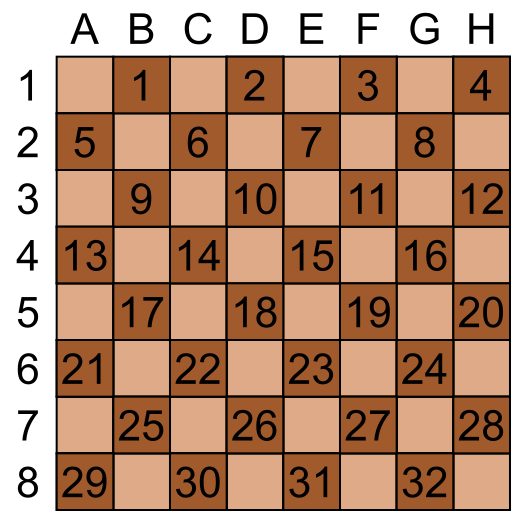
\includegraphics[scale=.6]{graphics/warcaby_planszaNumerowana.png}
    \caption{Numeracja pól i współrzędne planszy}
    \label{fig:numer}
\end{figure}


W przypadku podania błędnego wejścia, program poprosi gracza o ponowne wprowadzenie ruchu od zera. W momencie gdy rozgrywka miałaby się skończyć, program informuje o zwycięzcy i kończy działanie.

\subsection{Find}

Dostępne sygnatury wywołania programu:
\begin{itemize}
    \item Pierwsze uruchomienie algorytmu genetycznego (zalecane jeśli użytkownik chce utworzyć nową sesję algorytmu genetycznego od zera)
    \begin{enumerate}
        \item Liczebność populacji osobników [liczba naturalna podzielna przez 4]
        \item Liczba pojedynków osobnika w procesie selekcji [liczba naturalna, przy czym 0 oznacza pojedynek z każdym innym osobnikiem]
        \item Głębokość przeszukiwania w Minimaksie [liczba naturalna większa od zera]
        \item Współczynnik losowej selekcji osobników [liczba całkowita]
        \item Szansa na mutację [liczba wymierna z przedziału od~0 do~1]
        \item Rodzaj kryterium stopu [0 $\rightarrow$ czas (w sekundach); 1 $\rightarrow$ liczba iteracji]
        \item Limit dla kryterium stopu [liczba naturalna]
    \end{enumerate}
    \item Reaktywacja algorytmu genetycznego z wybranego pliku populacji
    \begin{enumerate}
        \item Nazwa pliku [ciąg znaków]
    \end{enumerate}
    \item Reaktywacja algorytmu genetycznego z ostatniego pliku populacji [BRAK ARGUMENTÓW]
    \vspace{1cm}
    \item Kontynuacja algorytmu genetycznego z nowymi parametrami
    \begin{enumerate}
        \item Nazwa pliku z którego należy wczytać populację [ciąg znaków]
        \item Liczba pojedynków osobnika w procesie selekcji [liczba naturalna, przy czym 0 oznacza pojedynek z każdym innym osobnikiem]
        \item Głębokość przeszukiwania w Minimaksie [liczba naturalna większa od zera]
        \item Współczynnik losowej selekcji osobników [liczba całkowita]
        \item Szansa na mutację [liczba wymierna między 0 a 1]
        \item Rodzaj kryterium stopu [0 $\rightarrow$ czas (w sekundach); 1 $\rightarrow$ liczba iteracji]
        \item Limit dla kryterium stopu [liczba naturalna]
    \end{enumerate}
\end{itemize}

Bezbłędne uruchomienie rozpocznie sesję algorytmu genetycznego z podanymi argumentami. W trakcie działania program operuje na plikach w katalogu \textit{heuristics} i jego podkatalogach: \textit{population} (pliki zapisanych populacji, z których można reaktywować sesje; program na bieżąco aktualizuje plik populacji) oraz \textit{output} (najlepiej przystosowany osobnik, tworzony w katalogu po osiągnięciu kryterium stopu). Oprócz tych podkatalogów istnieją również \textit{single} (katalog na samodzielne tworzenie plików ciągów wag) i~\textit{archive} (archiwum w którym można bezpiecznie zapisywać pliki ciągów wag), lecz program na tych dwóch podkatalogach nie wykonuje żadnych operacji oprócz ich stworzenia.

Sesja algorytmu genetycznego na bieżąco informuje o postępie - w każdej iteracji drukuje numer porządkowy obecnie ewaluowanej generacji oraz stosunek postępu do limitu we wcześniej podanym kryterium stopu (np. 5/100 generacji lub 100/2000 sekund). W razie niespodziewanego wcześniejszego zakończenia programu, możliwym jest odczyt argumentów sesji i postępu z pliku ostatniej populacji.

\subsection{Show}

Dostępne sygnatury wywołania programu:
\begin{itemize}
    \item Wydrukowanie ciągu wag z pliku osobnika
    \begin{enumerate}
        \item Ścieżka do pliku osobnika
    \end{enumerate}
\end{itemize}

Program drukuje listę opisanych parametrów z przydzielonymi im wagami z podanego pliku. Jest to użyteczne narzędzie do wglądu w wyniki sesji algorytmu genetycznego.


	\cleardoublepage
	
	\chapter{Testy}
\thispagestyle{chapterBeginStyle}

{\color{dgray}
W tym rozdziale omówione zostaną wyniki różnych sesji algorytmu genetycznego, badań, testów i porównań. Zostaną wyciągnięte wnioski na temat parametrów oceny heurystycznej które okażą się niepotrzebne lub zaniedbywalne. W miarę możliwości określona zostanie również siła algorytmu Minimax z wyznaczoną funkcją oceny. Porównane też zostaną wyniki algorytmu genetycznego z różnymi głębokościami przeszukiwań.
}

\textit{Na pewno prowadzący się ucieszy}


	\cleardoublepage
	
	\chapter*{Podsumowanie}
\addcontentsline{toc}{chapter}{Podsumowanie}
\thispagestyle{chapterBeginStyle}

W pracy przeprowadzono kilka sesji algorytmu genetycznego w~ramach eksperymentów na algorytmie Minimax z funkcją oceny heurystycznej. Udało się poznać częściowe odpowiedzi na zadane pytania i~sformułować z nich hipotezy.

Najważniejszym rezultatem testów jest uśredniony ciąg wag dla parametrów funkcji oceny. Dzięki niemu udało się określić parametry o~większym wpływie na rozgrywkę w warcabach i~odrzucić parametry niższego priorytetu. Podsumowano powstałą strategię jako agresywną taktykę dążącą do jak najszybszego awansu piona do damki. W~przyszłości można zapuścić sesję algorytmu genetycznego ze skróconą listą parametrów, aby uzyskać jeszcze dokładniejsze wagi.

Kolejnym ważnym wnioskiem jest różnica w perspektywach graczy MIN i~MAX. Okazuje się, że dobra strategia w warcabach (i~prawdopodobnie innych grach dwuosobowych o~sumie zerowej), opierająca się o~Minimaxa, powinna zwracać uwagę na to który gracz dokonuje wyboru spośród liści drzewa przeszukiwań. Wstępne eksperymenty pokazały, że taktyka pod MAXa jest na ogół bardziej ofensywna, natomiast taktyka pod MINa - bardziej defensywna.

Jednak mimo osiągnięcia zamierzonych celów, praca ta jest zaledwie początkiem bardziej rozbudowanych badań i projektów. Z racji iż kody źródłowe otwarte są na rozszerzenia oraz umieszczone są w repozytorium \textbf{GitHub}, dalsze wsparcie projektu jest jak najbardziej możliwe.

Przyjrzenie się bliżej perspektywom MINa i MAXa to naturalne rozszerzenie pracy. Może ono stanowić ciekawy wgląd w algorytmy decyzyjne, a nawet w teorię gier. Innym pomysłem na rozwój projektu jest zastosowanie przeróżnych optymalizacji bądź mechanizmów poprawiających decyzyjność Minimaxa, takich jak \textit{Quiescence Search}. Ponadto, można pomyśleć nad zintegrowaniem powstałego modelu sztucznej inteligencji z siecią internetową.


	\cleardoublepage
	
	
	%%%%%%%%%%%%%%%%%%%%%%%%%%%%%%%%%%%%%%%%%%%%%%%%%%%%%%%%%%%%%%%%%%%%%%%%%%%%%%
	%%%%%%%%%%%%%%%%%%%%%%%%%%%%%%% BIBLIOGRAFIA %%%%%%%%%%%%%%%%%%%%%%%%%%%%%%%%%
	%%%%%%%%%%%%%%%%%%%%%%%%%%%%%%%%%%%%%%%%%%%%%%%%%%%%%%%%%%%%%%%%%%%%%%%%%%%%%%

	\pagestyle{bibliographyStyle}
	\bibliographystyle{plabbrv}
	\bibliography{literatura}
	\thispagestyle{chapterBeginStyle}
        \addcontentsline{toc}{chapter}{Bibliografia}
	\cleardoublepage
	
	%%%%%%%%%%%%%%%%%%%%%%%%%%%%%%%%%%%%%%%%%%%%%%%%%%%%%%%%%%%%%%%%%%%%%%%%%%%%%%
	%%%%%%%%%%%%%%%%%%%%%%%%%%%%%%%%% DODATKI %%%%%%%%%%%%%%%%%%%%%%%%%%%%%%%%%%%%
	%%%%%%%%%%%%%%%%%%%%%%%%%%%%%%%%%%%%%%%%%%%%%%%%%%%%%%%%%%%%%%%%%%%%%%%%%%%%%%
	
	\appendix
	\pagestyle{appendixStyle}
       \renewcommand{\appendixname}{Załącznik}
	
	\chapter{Zawartość płyty CD}
\thispagestyle{chapterBeginStyle}
\label{plytaCD}

{\color{dgray}
W tym rozdziale należy krótko omówić zawartość dołączonej płyty CD.
}


	
	\cleardoublepage

\end{document}

